\documentclass[11pt]{article}

% Impostazioni del documento
\usepackage[a4paper,top=3cm,bottom=3cm,left=2cm,right=2cm,marginparwidth=2.5cm]{geometry}
\usepackage{parskip} % Spazio tra i paragrafi
\usepackage{setspace} % Interlinea
\onehalfspacing % Interlinea 1.5

% Impostazioni del font
\usepackage{mathptmx} % Times New Roman
\usepackage[T1]{fontenc}

% Altri
\usepackage{multicol}
\usepackage{graphicx}
\usepackage{enumitem}
\usepackage{amssymb}
\usepackage{xcolor}
\usepackage{float}
\usepackage{ntheorem}
\usepackage{mathtools}
\usepackage{amsmath}
\usepackage{makeidx}
\usepackage{subcaption}
\usepackage{hyperref}
\hypersetup{
    colorlinks=true,    % Rendi i link colorati
    linkcolor=blue,     % Colore dei link interni (es. sezioni)
    citecolor=blue,     % Colore delle citazioni bibliografiche
    urlcolor=blue       % Colore degli URL
}

% Definizione di un nuovo ambiente "definizione"
\theoremstyle{definition} \newtheorem{definizione}{Definizione}[section] % Questo numererà le definizioni all'interno di ogni sezione

\makeindex

\begin{document}

\begin{titlepage}
    \centering
    
\includegraphics[width=0.5\textwidth]{aau.png}
    \vfill
    \begin{center}
        {\LARGE Advance topics in CS \par}
        \vspace{0.5cm}
        {\large Alessandro Castelli [12246581] \par}
        \vspace{0.5cm}
        {\large \today \par}
    \end{center}
    \vfill
\end{titlepage}

\tableofcontents

\newpage


\section{The big picture}
    \subsection{Notation}
    \begin{itemize}
        \item \textcolor{red}{\textbf{$m$}} è il plaintext: \textcolor{red}{\textbf{$m$}} $\Leftarrow$ $M$
        \item \textcolor{black}{\textbf{$c$}} è il chipertext:  \textcolor{black}{\textbf{$m$}} $\Leftarrow$ $C$
        \item \textcolor{red}{\textbf{$sk$}} è la secret key:  \textcolor{red}{\textbf{$m$}} $\Leftarrow$ $K$
    \end{itemize}

    \begin{itemize}
        \item $ \text{Gen : K} \stackrel{\$}{\Rightarrow} \textcolor{red}{sk}$ 
        \item $ \text{Enc : M} \times K \rightarrow C$
        \item $\text{Dec : C} \times K \rightarrow M$
    \end{itemize}

    \subsection{Symmetric encryption}
    \begin{definizione}
        An encryption scheme in which the same key sk is used for both encryption and decryption
        is called symmetric encryp
    \end{definizione}

    \begin{definizione}
        Uno schema di encryption è corretto se: 
        \begin{equation}
            \forall m \in \text{M and } \forall \textcolor{red}{sk}  \in K \text{ : } Dec_{\textcolor{red}{sk}}(Enc_{\textcolor{red}{sk}}(m)) = m
        \end{equation}
    \end{definizione}

    \subsection{Let's revisit a game for secure encryption}
    \begin{figure}[H]
        \centering
        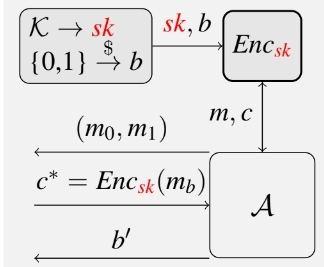
\includegraphics[width=0.4\linewidth]{1.jpg} 
        \caption{Encryption Function}\label{fig:Figura1}
    \end{figure}
    In riferimento alla Figura \ref{fig:Figura1}, consideriamo il gioco dell'indistinguibilità standard per la crittografia simmetrica.
    L'obbiettivo dell'avversario è distinguere tra la crittografia di $m_0$ e $m_1$.
    In pratica l'avversario deve essere in grado di carpire informazioni extra $L = f(m,c,\textcolor{red}{sk})$ ogni volta che un device accede alla chiave segreta.

    \subsection{Kerckhoffs' Principle}
    \begin{definizione}
        Il metodo di cifratura non deve essere necessariamente segreto e deve poter cadere nelle mani del nemico senza inconvenienti
    \end{definizione}

    Questo perchè un qualsiasi schema crittografico verrà prima o poi sottoposto a reverse engeneering.
    \newline
    \textbf{Basta una chiava molto grande per garantire la sicurezza?} La risposta è no, una chiava molto grande ci aiuta soltanto nel caso degli attacchi brute force ma non nei casi in cui l'attaccante ha informazioni aggiuntive.

\section{Crypto Engineering}
    \subsection{Crypto VS Security Engineering}
    La criptoingegneria è una sottoarea dell'ingegneria della sicurezza. La differenza principale sta nell'enfasi sul pensiero sistemico: è più forte nell'ingegneria della sicurezza che nella criptoingegneria. Quando gli ingegneri considerano i sistemi, tendono a concentrarsi sui componenti tecnici; ma ovviamente i sistemi sono costituiti anche da esseri umani; ci sono norme e regolamenti, incentivi, ecc. Oggi faremo una deviazione nel lato meno tecnico delle cose e considereremo il "fattore umano".

    \subsection{Usability as key requirements}
    Molti corsi sulle criptovalute iniziano molto presto con la revisione di alcuni principi proposti da Auguste Kerckhoffs. 
    Uno dei suoi principi chiave è: 
    \begin{quote}
     "Infine, date le circostanze in cui deve essere utilizzato, il sistema deve essere facile da usare e non deve essere stressante da usare o richiedere ai suoi utenti conoscere e rispettare un lungo elenco di regole"
    \end{quote} 
    Dovrebbe essere ovvio che sistemi complicati, fastidiosi o scomodi non verranno adottati nella pratica: le caratteristiche di sicurezza non utilizzate non contribuiscono realmente alla sicurezza.
    \newline
    Quindi che un sistema dovrebbe essere usabili è ovvio ma lo stesso principio dovrebbe adattarsi anche alle componenti crittografiche?

    \subsection{Types of errors}
    \begin{itemize}
        \item \textbf{Capability}: è più facile che commettiamo errori quando ci vengono assegnati compiti che vanno oltre le nostre capacità, inoltre gli esseri umani possono contrare la loro attenzione su un compito alla volta.
        \item \textbf{Human Factor}
    \end{itemize}

    Considera la situazione in cui i cassieri devono digitare il proprio ID e PIN/password alla cassa prima di utilizzarla. 
    Se non lavorano solo alla cassa, ma aiutano anche i clienti in negozio, l'ulteriore processo di accesso/disconnessione potrebbe rapidamente diventare una seccatura. 
    È facile immaginare che la regola del login quando si lavora alla cassa degeneri nella regola secondo cui "qualcuno" deve essere loggato. 
    Quindi una persona accede e non si disconnette mai, consentendo così a tutti (compresi eventuali avversari) di operare la cassa come e quando necessario. 
    In questo sistema il problema è quello degli incentivi. 
    Se, per ciascun lavoratore, le vendite totali attribuite al suo ID contassero (ad esempio) per un bonus alla fine di una giornata lavorativa, sarebbero più disposti a sopportare il fastidio di entrare e uscire.
    
    \subsection{Errors based on misunderstanding}
    \begin{figure}[H]
        \centering
        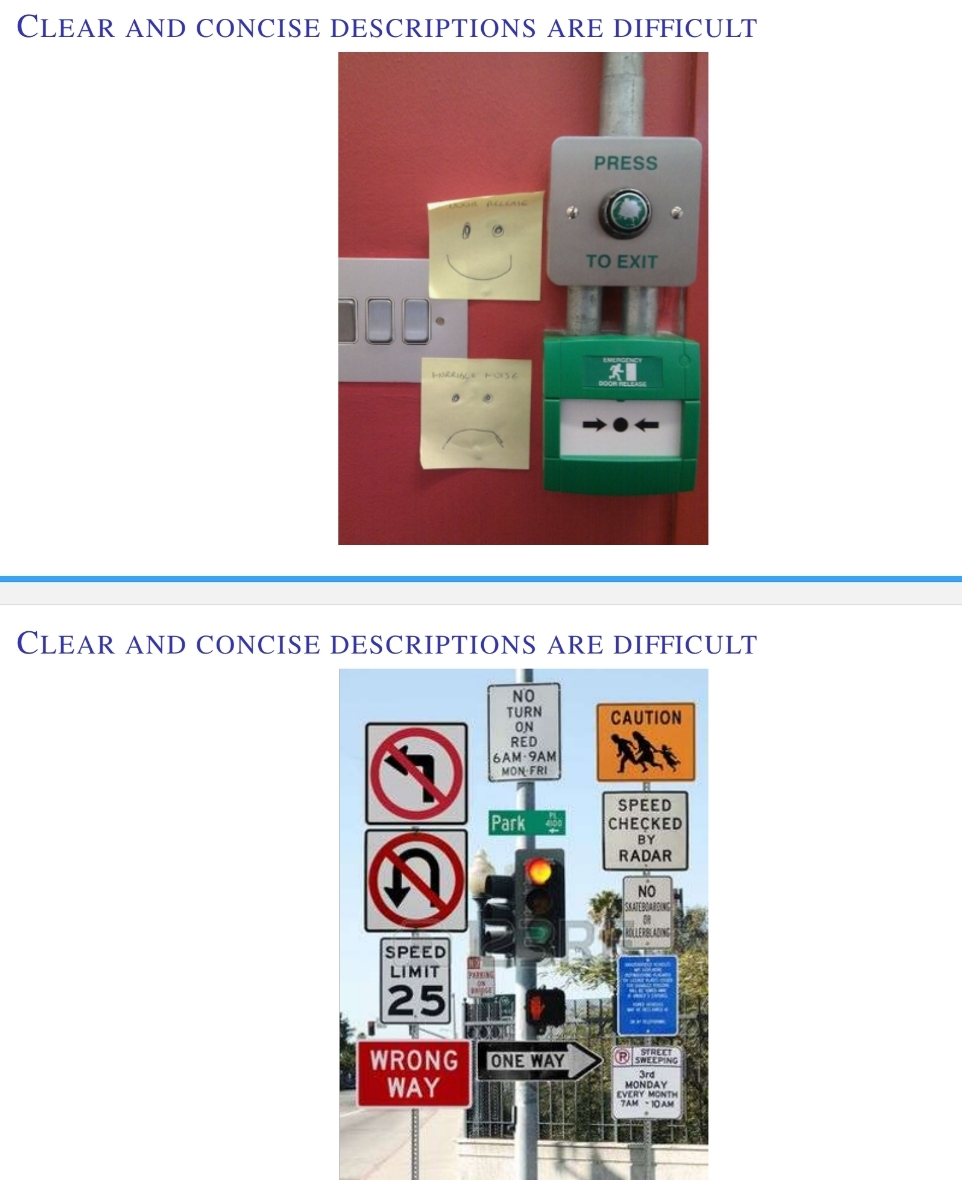
\includegraphics[width=0.4\linewidth]{2.jpg} 
        \caption{Example misunderstanding}\label{fig:figura2}
    \end{figure}

    Come puoi vedere dalla Figura\ref{fig:figura2} ci sono molti errori del genere che si possono verificare nella vita reale. 


    \subsection{Errors based on Risk taking}
    Un comportamento rischioso potrebbe essere visto come una violazione di alcune regole. 
    Reber la definì: 
    \begin{quote}
    "un'azione che mette a repentaglio qualcosa di valore”. 
    \end{quote}
    Il comportamento rischioso è qualcosa che è difficile da comprendere appieno. Un potenziale fattore che contribuisce è che il rischio è un’azione che nella società tipicamente porta a (forte) feedback negativo. 
    Ma ad alcune persone piace questo feedback avversivo (cioè la paura che viene fornito con esso fornisce una forma di eccitazione).
    Il corpo rilascia, come risposta fisiologica, un ormone chiamato adrenalina. L'adrenalina è anche associato all'euforia, e questo chiaramente fa sentire bene; 
    il ciclo di eccitazione (precedente), il brivido (durante) e l'euforia (dopo) associati all'assunzione di rischi possono essere sufficientemente gratificanti da diventare potenzialmente altamente assuefattivi.
    Un altro modo di intendere il rischio è come una caratteristica intrinseca della personalità di qualcuno: quello è una parte della propria struttura psicologica, in contrapposizione a un comportamento (che è stato appreso e può essere disimparato).
    Esiste anche il concetto di \textbf{“omeostasi del rischio”}. Ciò si riferisce all'osservazione che quando rendiamo una situazione più sicura, quindi le persone tendono a correre rischi maggiori, ma quando una situazione lo è percepito come pericoloso, le persone tendono a essere più attente.
    
    \subsection{Typical Miatakes when Using Crypto}
    Quest'anno alcuni ricercatori hanno sviluppato un nuovo strumento per scansionare le implementazioni crittografiche alla ricerca di vulnerabilità comuni.
    Hanno trovato un numero maggiore di app che presentano questi problemi.
    Hanno anche scoperto che alla maggior parte degli sviluppatori di app non importava.
    Alcune di esse le puoi vedere nelle Figure \ref{fig:figure_general}
    \begin{figure}[H]
        \centering
      
        \begin{subfigure}{0.48\textwidth}
          \centering
          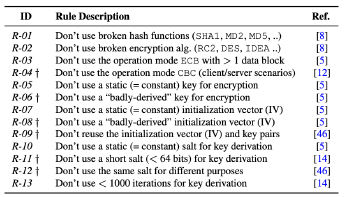
\includegraphics[width=\textwidth]{3.png}
          \caption{Vari problemi}
          \label{fig:figura3}
        \end{subfigure}
        \hfill
        \begin{subfigure}{0.48\textwidth}
          \centering
          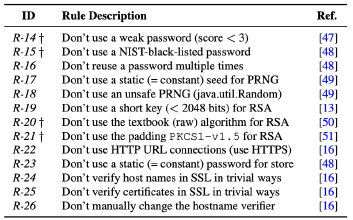
\includegraphics[width=\textwidth]{4.png}
          \caption{Vari problemi}
          \label{fig:figura4}
        \end{subfigure}
      
        \caption{Descrizione generale dei problemi}
        \label{fig:figure_general}
      
      \end{figure}
    
    \subsection{Making sense of terminology}
    Non importa cosa sviluppiamo (ad esempio una specifica, un'API, un software, un hardware), arriva il momento in cui dobbiamo garantire che \textit{la cosa faccia quello che dovrebbe}.
    Esistono numerosi termini che le persone utilizzano per indicare una serie di modi in cui significa "dovrebbe". Molte persone li usano in modo intercambiabile, la mia opinione su di loro è la seguente
    \begin{itemize}
        \item \textbf{Test}: dato un insieme di proprietà (ovvero casi di test), l'oggetto soddisfa le proprietà? (Stiamo costruendo la cosa correttamente?)
        \item \textbf{Convalida}: dati i requisiti, la “cosa” soddisfa i requisiti? (Siamo noi a costruire la “cosa” giusta?)
        \item \textbf{Verifica}: dato un insieme di definizioni formali, la “cosa” soddisfa queste definizioni? (Stiamo costruendo la “cosa” secondo le nostre specifiche?)
    \end{itemize}

    Molti prodotti richiedono una qualche forma di certificazione per dimostrare che soddisfano alcuni standard (minimi) prima di poter essere venduti.
    Molti prodotti utilizzano la certificazione per aumentare il loro valore di mercato.
    La valutazione precede la certificazione: solo se un prodotto supera un regime di valutazione può essere certificato. Durante la valutazione, un prodotto viene testato in base al regime di valutazione e ciò può richiedere ad es. una qualche forma di verifica (formale).
    I prodotti sensibili alla sicurezza (ad esempio il chip di una carta di credito o debito, terminali di punti vendita, ecc.) possono entrare nel marchio contrassegnato solo dopo la certificazione. Quindi per \textbf{certificazione} intendiamo una certificazione scritta che garantisce che il prodotto possieda almeno alcuni requisiti ben specifici.
    La certificazione è il processo di produzione di un “timbro di approvazione” riconosciuto; in genere un fornitore contatta un ente di certificazione (un ente governativo o un ente industriale) e un valutatore indipendente.
    La valutazione fa parte della certificazione: un laboratorio/azienda (indipendente) esegue una serie di test come richiesto nello schema di certificazione che sono allineati ad alcuni standard.
    Alcuni mercati/schemi seguono standard pubblici come la metodologia Common Criteria o FIPS 140-3, altri non sono completamente trasparenti.

    In genere una valutazione prevede tre parti che interagiscono tra loro:
    \begin{itemize}
        \item Venditore/Sponsor: il soggetto che desidera ottenere una certificazione di sicurezza per un prodotto
        \item Certificatore: istituzione che può emettere certificati di sicurezza
        \item Valutatore: un laboratorio di valutazione scelto dal fornitore
    \end{itemize}

    Gli organismi di certificazione in genere supervisionano il processo e interagiranno con il valutatore per garantire che ricevano un rapporto di valutazione sufficientemente dettagliato. Possono richiedere test aggiuntivi se lo ritengono opportuno.
    I valutatori spesso devono essere certificati per uno schema: devono cioè sottoporsi ad alcuni test
    prima che siano accettati dai Certificatori.

    \subsection{Types of Security Certification Schemes}
        Per ora guardali dalle slides, in ogni caso non dicono molto di interessante.
    
\section{Making Symmetric Crypto}
    \subsection{AES: The Advanced Encryption Standard}
    Il cifrario a blocchi AES è un cifrario prodotto, trasforma il testo in chiaro in testo cifrato mediante l'uso iterato di alcune round functions
    Le funzioni round AES formano una rete di sostituzione-permutazione.   
    Noi considereremo AES-128:che prende chiavi da 128 bit ed anche il plaintext e il ciphertext sono grandi 128 bit.
    Inoltre tieni in mente che: AES utilizza il campo finito $F_{2^8}[X]/X^8 + X^4 + X^3 + X + 1$. Gli elementi di questo campo rappresentano byte con operazioni non standard su di essi. Le operazioni di addizione, moltiplicazione e divisione, denotate rispettivamente da $\oplus$, $\cdot$, e $\div$, seguono le regole del campo $F_{2^8}$.

    \begin{itemize}
      \item \textbf{Elementi del Campo:} Gli elementi del campo possono essere trattati come byte, ma le operazioni seguono regole specifiche del campo finito.
      \item \textbf{Operazioni di Campo:} L'addizione, moltiplicazione e divisione sono effettuate secondo le regole del campo finito $F_{2^8}$.
      \item \textbf{Costanti del Campo:} La costante $03_{16}$ rappresenta l'elemento $X + 1$ nel campo finito.
      \item \textbf{Matrici di Elementi del Campo:} AES opera su matrici di elementi del campo finito. Le operazioni sono eseguite su queste matrici, leggendo gli elementi colonna per colonna.
    \end{itemize}

    \subsection{Come Funziona AES}

        AES (Advanced Encryption Standard) è una cifra a blocchi che crittografa dati in blocchi di dimensione fissa, con una dimensione di blocco di 128 bit. Ecco una panoramica di alto livello di come funziona AES:

        \subsubsection*{Ingresso e Chiave}
        \begin{itemize}
        \item \textbf{Plaintext:} I dati in chiaro da cifrare sono divisi in blocchi da 128 bit.
        \item \textbf{Chiave:} La chiave segreta è anch'essa di 128 bit.
        \end{itemize}

        \subsubsection*{Generazione delle Chiavi di Round}
        \begin{itemize}
        \item La chiave segreta viene espansa in una serie di sottochiavi attraverso un processo noto come Key Expansion.
        \end{itemize}

        \subsubsection*{AddRoundKey}
        \begin{itemize}
        \item Ogni blocco di dati in chiaro viene combinato con una sottochiave iniziale attraverso un'operazione di XOR, nota come AddRoundKey.
        \end{itemize}

        \subsubsection*{Round}
        \begin{itemize}
        \item L'algoritmo esegue una serie di round, ciascuno composto da diverse operazioni:
            \begin{itemize}
            \item \textbf{SubBytes:} Sostituisce ogni byte del blocco in chiaro con un valore dalla S-box.
            \item \textbf{ShiftRows:} Scorre le righe del blocco.
            \item \textbf{MixColumns:} Combina i dati nelle colonne del blocco.
            \item \textbf{AddRoundKey:} XOR del blocco risultante con la sottochiave corrente.
            \end{itemize}
        \end{itemize}

        \subsubsection*{Round Finale}
        \begin{itemize}
        \item L'ultimo round differisce dagli altri poiché non include l'operazione MixColumns.
        \end{itemize}

        \subsubsection*{Output}
        \begin{itemize}
        \item Il risultato finale di tutti i round è il blocco cifrato.
        \end{itemize}

    \subsection{Random Numbers}
    Il concetto di casualità è familiare a molti di noi, ma ciò può implicare fraintendimenti sul suo significato matematico effettivo.

    Innanzitutto, un singolo numero non può essere casuale di per sé. Solo un processo mediante il quale selezioniamo ripetutamente numeri può avere la proprietà di selezionare numeri casuali.

    In secondo luogo, "casuale" non è la stessa cosa di "arbitrario". Considera, ad esempio, l'istruzione "premere un tasto qualsiasi". Questa istruzione significa che può essere selezionato qualsiasi tasto sulla tastiera. Se questa istruzione viene ripetuta, un utente potrebbe premere sempre il tasto con etichetta "a". Al contrario, l'istruzione "premere un tasto casuale" implicherebbe che, ripetendo questa istruzione, l'utente dovrebbe selezionare casualmente un tasto, e quindi premere sempre lo stesso tasto non sarebbe accettabile.

    possiamo dedurre che il concetto di casualità implica che stiamo parlando di un processo che coinvolge un insieme di elementi e che, alla ripetizione del processo, è impossibile conoscere quale sarà l'esito della successiva invocazione dato quanto appreso da tutte le invocazioni precedenti.

    Quindi, dato un insieme e una distribuzione su quest'ultimo, estrarre un elemento da questo insieme in modo casuale significa che:
    \begin{itemize}
    \item Nel corso di molteplici estrazioni di elementi, la distribuzione degli elementi estratti è indistinguibile dalla distribuzione dell'insieme sottostante (gli elementi sembrano "imparziali").
    \item La probabilità di estrarre qualsiasi elemento è indipendente dagli elementi precedentemente estratti (gli elementi sono "imprevedibili").
    \end{itemize}

    Abbiamo scelto il nostro insieme di numeri come bit ${0, 1}$, con probabilità $p(0) = p(1) = 0.5$. Quindi, in un esperimento in cui estraiamo bit casuali da questo insieme, ci aspettiamo che (in una serie sufficientemente lunga), tutti i bit campionati abbiano nuovamente la distribuzione $p(0) = p(1) = 0.5$. Ci aspetteremmo anche che qualsiasi sequenza di bit come 00, 01, 10, 11 si verifichi con la stessa probabilità (cioè 0.25 in questo caso).

    Se i singoli bit campionati (su una sequenza sufficientemente lunga) sono equiprobabili e qualsiasi sequenza di essi è equiprobabile, allora i bit sarebbero imparziali. Se possiamo anche dimostrare che le sequenze sono indipendenti, allora i bit campionati sarebbero anche imprevedibili.

    \textbf{Se utilizziamo numeri casuali per generare chiavi}, in questo caso abbiamo veramente bisogno sia di imparzialità che di imprevedibilità.

    \textbf{Se utilizziamo numeri casuali come valori di inizializzazione (IVs)}, allora abbiamo bisogno sia di imparzialità che di imprevedibilità.

    \textbf{Per i numeri utilizzati come nonce}, abbiamo bisogno di imparzialità, ma non necessariamente di imprevedibilità.

        \subsubsection*{Hot to create Random Numbers}
        \begin{quote}
        Chiunque tenti di generare numeri casuali con mezzi deterministici vive, ovviamente, in uno stato di cattiva salute mentale. — John von Neumann
        \end{quote}
        
        Il criterio dell'"imprevedibilità" richiede di riflettere un po':
        \begin{itemize}
        \item Se un avversario avesse un potere computazionale illimitato (ossia, le stesse assunzioni che abbiamo ipotizzato per la "sicurezza incondizionata"), allora, naturalmente, von Neumann ha ragione e non c'è modo per noi di produrre numeri casuali algoritmici.
        \item Se non assumiamo che un avversario abbia un potere computazionale illimitato, potremmo forse formulare un concetto di "indistinguibilità computazionale" in cui speriamo che un avversario non possa distinguere una data sequenza di numeri da una sequenza di numeri veramente casuali (con la loro potenza computazionale).
        \item Da dove otterremmo numeri veramente imprevedibili?
        \end{itemize}

        \textbf{Generatore Pseudo-casuale (PRNG):} In un contesto asintotico (ossia, considerando sequenze sufficientemente lunghe), una funzione è un PRNG se il suo output è computazionalmente indistinguibile dalla vera casualità.

        \textbf{Generatore Casuale Reale (TRNG):} È un generatore basato su un processo intrinsecamente probabilistico e sufficientemente complesso da essere imprevedibile.

        Esistono una serie di fonti di vera casualità basate su processi fisici, ed è imperativo verificarne la distribuzione (nella crittografia spesso abbiamo bisogno di distribuzioni uniformi). È anche importante garantire che non possano essere manipolate.

        A seconda dell'applicazione, sono disponibili diverse fonti di casualità naturale:
        \begin{itemize}
        \item il tempo trascorso tra l'emissione di particelle durante il decadimento radioattivo;
        \item il rumore termico da un diodo semiconduttore o una resistenza;
        \item l'instabilità di frequenza di un oscillatore a funzionamento libero;
        \item la quantità di carica di un condensatore metallo-isolante-semiconduttore durante un periodo fisso di tempo;
        \item il suono da un microfono o l'input video da una telecamera; segnali provenienti da un'antenna.
        \end{itemize}

        Alcune fonti richiedono attrezzature specializzate e non possono essere incorporate su dispositivi di consumo; alcune fonti possono essere manipulate dagli avversari e quindi richiedono una considerazione speciale.

        Prodotti di sicurezza di alta qualità includeranno tipicamente un TRNG hardware (spesso basato su oscillatori a funzionamento libero).

        Alcuni esempi per avere delle stringhe di numeri casuali sono le \textbf{claudflare lava lampa} (Figure \ref{fig:figura5}): Cloudflare ha disposto circa 100 lampade lava su uno dei muri nella hall della sede di Cloudflare e ha posizionato una telecamera puntata sulle lampade. La telecamera scatta foto delle lampade a intervalli regolari e invia le immagini ai server di Cloudflare. Tutte le immagini digitali vengono realmente memorizzate dai computer come una serie di numeri, con ogni pixel che ha il proprio valore numerico. Così, ogni immagine diventa una sequenza di numeri totalmente casuali che i server di Cloudflare possono utilizzare come punto di partenza per la creazione di chiavi di crittografia sicure.

        \begin{figure}[H]
            \centering
            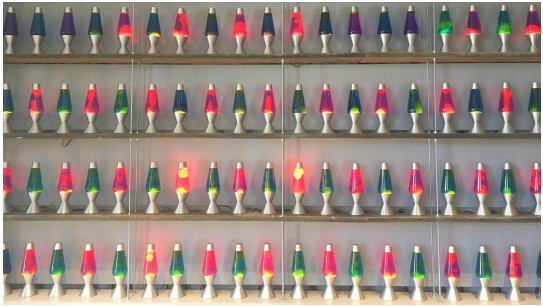
\includegraphics[width=0.4\linewidth]{5.png} 
            \caption{Cloudflare lava lamp}\label{fig:figura5}
        \end{figure}

        Anche \textbf{RANDOM.ORG} offre numeri casuali reali a chiunque su Internet. La casualità proviene dal rumore atmosferico, che per molti scopi è migliore rispetto agli algoritmi pseudo-casuali tipicamente utilizzati nei programmi informatici. Le persone utilizzano RANDOM.ORG per effettuare estrazioni, lotterie e concorsi, per gestire giochi online, per applicazioni scientifiche e per arte e musica.
        
        Non tutti i sistemi dispongono di generatori di numeri casuali reali (TRNG) hardware dedicati e, pertanto, le persone hanno suggerito varie soluzioni alternative (tratte dal capitolo 5 di HAC):
        \begin{itemize}
        \item l'orologio di sistema;
        \item il tempo trascorso tra la pressione dei tasti o i movimenti del mouse;
        \item il contenuto dei buffer di input/output;
        \item l'input dell'utente;
        \item valori del sistema operativo come il carico di sistema e le statistiche di rete.
        \end{itemize}

        Chiamo queste fonti "delicate" perché possono essere potenzialmente facilmente manipolate dagli avversari (che possono eseguire un processo sulla macchina di destinazione). Inoltre, alcuni di questi processi non sono davvero casuali come nell'accezione di imprevedibili (pensa all'orologio di sistema: cambia in modo piuttosto prevedibile).

        I sistemi operativi generalmente raccolgono dati da "tutte" queste fonti per creare un pool di casualità da cui le applicazioni possono attingere alcuni "bit" casuali. Un'analisi della strategia di generazione di numeri casuali in Linux può essere trovata qui: \url{https://web.archive.org/web/20081003041432/http://www.pinkas.net/PAPERS/gpr06.pdf}.
        
        Ogni TRNG "raccoglie" entropia nel tempo; pertanto, solo una volta che è stata generata a sufficienza entropia, è possibile chiedere effettivamente al TRNG di generare un numero casuale (ossia, una sequenza di bit di una lunghezza specificata).

        Tuttavia, molte applicazioni crittografiche richiedono "molta" casualità: ad esempio, per nuove chiavi di sessione (cifratura autenticata) più eventualmente un vettore di inizializzazione (IV); e poi lo stesso ogni volta che avviene una ricreazione delle chiavi.

        Quindi, nella pratica, utilizziamo un TRNG per generare il seme per un PRNG: quest'ultimo quindi produce pseudo-casualità rapidamente.

        Un modo semplice di generare numeri pseudo-casuali è utilizzare qualche forma di congruenza lineare (ossia, un'equazione semplice su un gruppo/anello/campo finito). Questo spesso porta a qualcosa chiamato LFSR (registro a scorrimento a retroazione lineare).

        Il problema con questo approccio è che i numeri risultanti non sono imprevedibili (neanche per un avversario con limitate risorse computazionali); anche se per LFSR opportunamente scelti, i numeri risultanti sono imparziali (quindi sono utili per test e sperimentazioni). Quindi, per la crittografia, dobbiamo cercare strategie di progettazione più complesse e, forse non sorprendentemente, possiamo riutilizzare alcune primitive crittografiche per costruire generatori di numeri pseudo-casuali crittograficamente sicuri.

        HMAC: codice di autenticazione basato su una funzione di hash, DRBG: generatore di bit pseudo-casuali deterministico. Una stringa di bit casuali fornisce quindi un numero casuale. HMAC-DRBG è HMAC in modalità OFB. Il seme è preso da qualche TRNG. La chiave è o fissa tra gli utenti (non praticabile) o la chiave di sessione è generata/scambiata parallelamente.

        HASH-DRBG utilizza una funzione di hash in modalità di contatore. Il seme è preso da qualche TRNG. Il contatore viene incrementato e alcune informazioni (incluso l'hash dalla chiamata precedente) vengono aggiunte prima che possa essere utilizzato come seme.

        Simile alle costruzioni basate su una funzione di hash, è anche possibile utilizzare un cifrario a blocchi in una modalità di operazione per creare casualità. NIST raccomanda di utilizzare AES o Triple-DES (e mette in guardia riguardo al secondo a causa della sua dimensione del blocco troppo piccola).

        NIST ha definito più DRBG, uno basato sul problema del DL (Discrete Logarithm) sulle curve ellittiche. La crittografia a curve ellittiche era destinata a sostituire la crittografia basata su RSA e DL convenzionale perché il problema DL su una curva ellittica può essere sostanzialmente più difficile e quindi si possono utilizzare chiavi più brevi per ottenere lo stesso livello di difficoltà rispetto a quando si usa RSA/DL. Ma questo particolare DRGB non era più veloce di altri DRGB e la NSA ha "corrotto" RSA Labs (all'epoca una grande e influente azienda nel settore della sicurezza informatica) per rendere questo DRGB la loro scelta "predefinita".
        Ciò sembrava sospetto perché già nel 2006 i ricercatori hanno evidenziato che i numeri casuali da questa costruzione erano effettivamente leggermente imparziali: \url{https://eprint.iacr.org/2006/190}.

        Ma successivamente alcuni altri ricercatori hanno dimostrato un possibile attacco che potrebbe implicare un backdoor deliberato. La costruzione (scheletrica) può essere delineata come segue. Siano P e Q punti su una curva ellittica su qualche campo finito adeguato; sia $s_i$ lo stato corrente e $x()$ la funzione che estrae la coordinata x da un punto EC, e $x_{16}$ la funzione che estrae tutti tranne 16 bit dal punto EC. La costruzione EC doppia procede quindi come segue:
        \[s_{i+1} = x(s_iP)\]
        \[o_i = x_{16}(s_iQ)\]

        Ora consideriamo questo come un attacco: si assume che l'avversario abbia selezionato i punti P e Q con attenzione in modo che \(dQ = P\). Mantengono d segreto ma spingono P e Q a essere i parametri pubblici in un'implementazione.
        Ora qualcuno utilizza questa costruzione con un seme iniziale \(s_0\) sconosciuto all'avversario.
        Ma l'avversario può vedere l'output \(o_i\) in qualche punto. Questo implica che conoscono tutti tranne 16 bit della coordinata x di \(s_iQ\). Pertanto, possono enumerare tutte le possibilità per questa coordinata x e testare quali di esse portano a punti effettivi sulla curva EC (ossia, quali di esse hanno una coordinata y valida). Otterranno un insieme di punti EC candidati. Per ciascuno di questi candidati possono calcolare lo stato successivo perché \(ds_iQ = s_iP\).
        Quando ottengono informazioni sullo stato successivo tramite \(o_{i+1}\), possono effettivamente confermare qual era il candidato corretto e con ciò conoscono lo stato attuale del RNG. Di conseguenza, possono prevedere tutti gli stati successivi fino a quando il RNG viene ricaricato.

        Quindi, perché questo suggerisce l'esistenza di una backdoor?
        Nello standard NIST, alcuni punti P e Q sono specificati, ma nessuno sa da dove provengano questi punti. E poiché il problema del DL su una curva ellittica è difficile, non possiamo verificare se esiste effettivamente un \(d\) tale che \(dQ = P\).
        NIST ha anche riconosciuto i contributi apportati dalla NSA a questo standard.
        Pertanto, c'è l'opinione ampiamente condivisa che la costruzione fosse intenzionale e parte dello sforzo più ampio della NSA per minare gli standard crittografici.
        Il nome in codice dell'operazione della NSA per minare gli standard crittografici è "Bullrun": \url{https://en.wikipedia.org/wiki/Bullrun_(decryption_program)} (grazie a Edward Snowden).
        Per ulteriori informazioni, consulta \url{http://dualec.org/}.


\end{document}
